\section{Теория}
\subsection{Уравнения Лагранжа}
Для моделирования падния фигуры я составил уравнения лагранжа второго рода.
В общем случае уравнение выглядит так:
\begin{equation}
\frac{d}{dt}\left(\frac{\partial L}{\partial \dot{q_i}} \right)-\frac{\partial L}{\partial q_i}=0,\qquad i=1,\dotsc,n;
\end{equation}
$q_i$~--- обощенные координаты, а L~--- кинетический потенциал~(или функция Лагранжа). $L=T-P$~  где T~--- кинетическая энергия, P~--- потенцияальная энергия, g~--- ускорение свободного падения.
\begin{equation}
T=\sum_{i} \frac{1}{2}m_i V_i^2+\sum_{i} \frac{1}{2}\omega_i^2 I_i.
\end{equation}
\begin{equation}
P=\sum_{i} m_i g_i h_i.
\end{equation}
В уравнениях (2) и (3) $m_i$~--- массы i-тых ребер, $V_i$~--- скорости i-тых точек, $\omega_i$~--- угловые скорости точек, $I_i$~--- моменты инерции~(которые вычисляются по формуле:~ $I_i=\frac{1}{1}m_i l_i^2$, где l~--- длина стержня между точками).
\subsection{Конкретный случай}
Для простоты рассказа будем использовать такой случай:~ на вход получено четыре точки, которые соединены тремя точками.
\begin{figure}[h!]
	\centering
	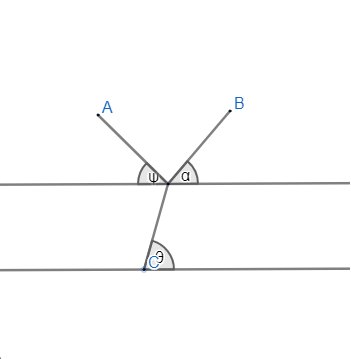
\includegraphics[width=200px, height=200px]{rogatka.png}
	\caption{Типовая фигура}
\end{figure} 
На вход подаются координаты точек A, B, C, O, а также матрица связей (она же матрица весов ребер).  В данном случае матрица выглядит таким образовм:
\[ edges = \bordermatrix{
        & A & B & C & O \cr
    A   & 0 & 0 & 0 & 1 \cr
    B   & 0 & 0 & 0 & 1 \cr
    C   & 0 & 0 & 0 & 1 \cr 
    O   & 0 & 0 & 0 & 0 \cr
}
\]
\par Уравнения Лагранжа в данном случае будут выглядеть так:
\begin{eqnarray}
\frac{d}{dt}\left(\frac{\partial L}{\partial \dot{\theta}} \right)-\frac{\partial L}{\partial \theta} & = & 0 \\ 
\ \frac{d}{dt}\left(\frac{\partial L}{\partial \dot{\phi}} \right)-\frac{\partial L}{\partial \phi} & = & 0 \\
\ \frac{d}{dt}\left(\frac{\partial L}{\partial \dot{\psi}} \right)-\frac{\partial L}{\partial \psi} & = & 0 \\
\ \frac{d}{dt}\left(\frac{\partial L}{\partial \dot{x}} \right)-\frac{\partial L}{\partial x} & = & 0 \ 
\end{eqnarray}
После подстановки подстановки всех значений в формулу, вычисления частных производных и упрощения, запишем систему (4) в матричном виде~ (левая часть в дальнейшем~---\textbf{ матрица А}, правая часть~--- \textbf{вектор b}):
\[\frac{d}{dt}\left( \begin{array}{cccc}
l_c^2\left(m_a + m_b \right)+I_c& 0 & 0 & \l_c\left(m_a + m_b\right)\\
        0           &       I_B         &       0       &       0 \\
        0           &       0         &       I_A        &       0 \\
l_c\left(m_a + m_b \right)& 0 & 0 & m_a + m_b + m_c        
\end{array}\right) = 
- \left( \begin{array}{c}
\cos{\theta}\left( m_a g l_c  + m_b g l_c + m_c g \frac{l_c}{2}\right) \\
 m_b g \frac{l_b}{2} \cos{\phi} \\
 m_a g \frac{l_a}{2} \cos{\psi} \\
  0
\end{array}\right)
\]
\subsection{Приближенное вычисление положения точек}
В общем случае, за каждый шаг мы приближенно вычисляем приращения с помощью системы (4)-(7):   
\begin{equation}
A^{-1} b =\Delta\dot {q}
\end{equation}
Затем пересчитывается вектор скоростей:
\begin{equation}
\vec V=\vec V+\Delta\dot{q}
\end{equation}
И, наконец, по вектору скоростей обновляются координаты точек. Осуществляются необходимые повороты и переносы точек.
%В программе положение точек пошагово обновляется 



